\section{Introduction}

Radiation therapy is now a reliable treatment for oncology.
Despite this consensus, the way to deliver radiotherapy for its best result remain very dependent upon doctors.
Moreover, it appears that there is a large variability across centers.

To achieve the best treatment, doctors need to solve a complex inverse mathematical optimization problem with multiples trade-offs.
There is a lack of standardized prioritization of constraints make the optimization a real challenge.
The standard procedure nowadays is to manually guide computer optimization: dosimetrists manually update the settings of an optimizing software (so called Treatment Planning System).


As this is very new and ongoing research, we generated synthetic phantom patients and associated trust-able clinical dose.
In future work, we hope to be able to apply this technique to real cases.

\section{Materials and Methods}

This is how you add one \cite{Pivot2023} or multiple citations \cite{Saporta2022,Robert2022}.

% example equation
And this is a dummy equation
\begin{equation}
I_\alpha = \int_0^\alpha f(x) dx
\end{equation}

% example two column figure (use figure instead of figure* for one column figure)
\begin{figure*}
  \centering
  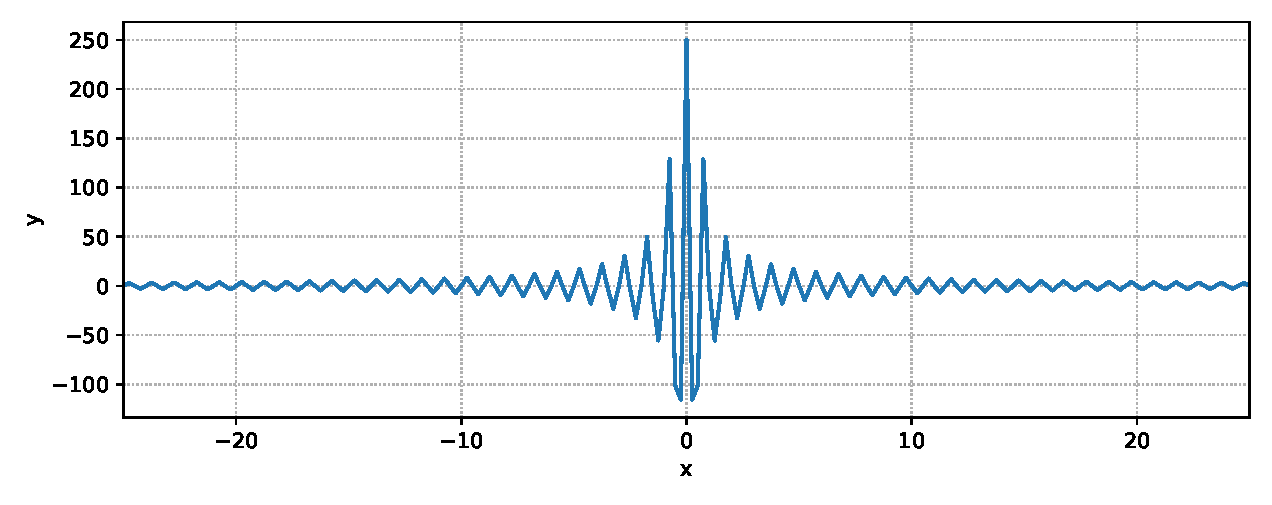
\includegraphics[width=1.0\textwidth]{./fig1.pdf}
  \caption{This a dummy figure to be replaced.}
  \label{fig:dummyfigure}
\end{figure*}

Figure \ref{fig:dummyfigure} shows how to include a figure.
Table \ref{tab:dummytable} shows how to include a table.

\bigskip

\lipsum[2-7]

\section{Results}
\subsection{Simulation results}

\lipsum[2-3]

\subsection{Other results}
\lipsum[2-3]

% example table
\begin{table}
  \centering
  \begin{tabular}{lrrr}
  \toprule
  $\alpha$   & $\beta$ & $\gamma$ & $\delta$ \\
  \midrule
  A          & 1       & a        & 3        \\
  B          & 2       & b        & 2        \\
  C          & 3       & c        & 1        \\
  \bottomrule
  \end{tabular}
  \caption{This is a dummy table to be replaced.}
  \label{tab:dummytable}
\end{table}



\section{Discussion}
\lipsum[2-9]


\section{Conclusion}
\lipsum[2]


